\documentclass[8pt, handout=show,notes=show]{beamer}

\usepackage[utf8x]{inputenc}
\usepackage[T1]{fontenc}
\usepackage{wrapfig}
\usepackage{default}
\usetheme[width=2cm]{Goettingen}
\usepackage{amsmath}
\usecolortheme{rose}
\usepackage{enumerate}
\usepackage{graphicx}
\usepackage{wrapfig} 
\usepackage{amsmath}
\usepackage{lmodern}

% \usepackage[colorlinks=true,urlcolor=blue,citecolor=green,linkcolor=blue,bookmarks=true]{hyperref}
\usepackage[french]{babel}
\author[]{Simon Carrignon \\ 
\vfill Encadrant: Nicolas Bred\`{e}che }
\institute[]{
	École~Pratique~des~Hautes~Études, \and TAO/LRI\\
	\pgfdeclareimage[height=0.5cm]{ephe}{images/logo_ephe_large.jpg} %declare logo image with an alias here 
	\pgfuseimage{ephe} \hfill \pgfdeclareimage[height=0.5cm]{inria}{images/taologo.jpg} %declare logo image with an alias here 
	\pgfuseimage{inria}
	
}

\usepackage[small]{caption}
% \DeclareLanguageMapping{american}{american-apa}
% \setbeamertemplate{caption}[numbered]
% \usepackage{subcaption}

% \usepackage{tikz}
% \usetikzlibrary{decorations.pathreplacing}
\useoutertheme{infolines}
% \logo{\includegraphics[height=0.5cm]{images/logo_ephe_large.jpg}}
% 	\usepackage{wrapfig}
\usepackage{subfigure}
\usepackage[footheight=1em]{beamerthemeboxes}

\addfootboxtemplate{\color{black}}{\color{white}
\hspace{2em}Simon Carrignon \hfill\insertframenumber/\inserttotalframenumber\hspace{2em}\null}

\title{Auto-organisation dans un essaim d'agents autonomes : \'{e}mergence de sp\'{e}cialisation}

\usepackage{algorithm}
\usepackage{algorithmic}

\usepackage[]{natbib}
\bibpunct{[}{]}{,}{a}{,}{,}
%%NOTES: DOCUMENT DE TRAVAIL ENTAMÉ LE 9 juin  2011
%%Talk fait a l'EPHE le 16 juin 2011. 
\date{$16$ Juin 2011}
\begin{document}
\begin{frame}
\maketitle

	\end{frame}
	
	%%%------------------------------------------------------------------------
	%%%----------------------------------------------------------------------
	\section{Introduction}
	%%%----------------------------------------------------------------------
	\begin{frame}{Contexte et motivation}
	\begin{figure}
	\includegraphics[height=3cm]{images/symbrion-gc1b.png}
	\end{figure}
	\begin{block}{Contexte}
		Essaims d'agents autonomes, capacités limitées, environnements inconnus et imprévisibles.
	\begin{itemize}
		\item Robotique évolutionnaire et évolution embarquée {\scriptsize \texttt{[Nolfi00, Watson99]}}.
% 		\item \'{E}volution \emph{open-ended} (bedau,ray).
	\end{itemize}
	\end{block}
	
% 	\begin{beamerboxesrounded}{test}
% 	 ×test
% 	\end{beamerboxesrounded}

	
	
	\begin{columns}
		\column{.5\textwidth}

	\begin{alertblock}{Question :}
	\'{E}mergence spontanée et non supervisée de sous-groupes spécialisés ?
	\end{alertblock}
	\end{columns}

% 	Artificial life and Embodied robotic
	
	%         \begin{itemize}
	% 		\item Bio-inspired solutions \citep{garnier07biolprinswarinte}
	% 		\item evolutionary robotic \citep{nolfi00evolrobobiolintetechselfmach}
	% 		\item embodied and unsupervised evolution \citep{watson02emboevoldistevolalgopopurobo}
	%         \end{itemize}
	
	\end{frame}
	
	\section{Description de mEDEA}
	%%%----------------------------------------------------------------------
	%%%----------------------------------------------------------------------
	%%%%%%%%%%%%%%%%%%%%%%%%%%%%%%%%%%%%%%%%%%%%%%%%%%%555
%From jm and nicolas frame 

  \newcommand{\mEDEA}{

	\begin{itemize}
		\item Chaque agent contient:
		\begin{itemize}
			\item un génome actif, utilisé pour contrôler l'agent,
			\item Une \emph{liste des génomes re\c cus}, utilisée pour stocker les génomes re\c cus pendant une génération,  
		\end{itemize}
		
		\item \`{A} chaque pas de temps, chaque agent :
		\begin{itemize}
			\item émet des copies dont son génome actif,
			\item stocke les génomes re\c cus des agents voisins.
		\end{itemize}
		
		\item \`{A} la fin d'une génération, chaque agent:
		\begin{itemize}
			\item "oublie" son génome actif, 
			\item choisit au hasard un génome parmis les génomes de sa \emph{liste de génomes re\c cus} comme nouveau génome actif et le mute légèrement,
			\item vide sa liste des génomes re\c cus.
		\end{itemize}
	\end{itemize}

}


%------------------------------------------------------------
\begin{frame}{L'algorithme <<mEDEA>>}
\begin{figure}
 \includegraphics[height=3cm]{images/medea0}
\end{figure}

  \mEDEA

\end{frame}

%------------------------------------------------------------
\begin{frame}{L'algorithme <<mEDEA>>}\addtocounter{framenumber}{-1}
\begin{figure}
 \includegraphics[height=3cm]{images/medea1}
\end{figure}
   \mEDEA
\end{frame}
%------------------------------------------------------------
\begin{frame}{L'algorithme <<mEDEA>>}\addtocounter{framenumber}{-1}
\begin{figure}
 \includegraphics[height=3cm]{images/medea2}
\end{figure}
   \mEDEA
\end{frame}

%------------------------------------------------------------

\begin{frame}{L'algorithme <<mEDEA>>}\addtocounter{framenumber}{-1}
\begin{figure}
 \includegraphics[height=3cm]{images/medea3}
\end{figure}
   \mEDEA
\end{frame}


%%%%%%%%%%%%%%%%%%%%%%%%%%%%%%%%%%



	
	%%%----------------------------------------------------------------------
	%%%----------------------------------------------------------------------
	\begin{frame}{Travaux précédents}
	\begin{columns}
	\column{0.5\textwidth} 
	\begin{figure}%[h]
	\includegraphics[width=\textwidth,height=3cm]{images/roborobo-setup-twosuns}
	\end{figure}
	\column{0.5\textwidth} 
	\begin{figure}%[h]
	\includegraphics[width=\textwidth,height=3cm]{images/medea-RealRobots}
	\end{figure}
	\end{columns}
	
	\vfill
	
% 	Travaux précédents
	\begin{itemize}
	\item Robuste aux changements environnementaux {\small[PPSN2010]}, \nocite{bredeche11mcmds} 
	\vfil
	\item Fonctionne sur robots réels {\small[MCMDS2011]}, %\nocitep{montanier}
	\vfil
	\item \'{E}mergence de l'altruisme {\small[ECAL2011]},
	\vfil
	\item \'{E}mergence de concensus {\small[MCMDS2011]}.
	\end{itemize}
	
% 	\vfill
	
	\end{frame}
	%%%----------------------------------------------------------------------
	%%%----------------------------------------------------------------------
	
% 	\subsection{Spéciation et spécialisation}
	
	%%%----------------------------------------------------------------------
	%%%----------------------------------------------------------------------
	
	\begin{frame}{Cadre et Problématique}
% 			\begin{columns}
			 
% 			\column{.5\textwidth}
			Spécialisation :
			\begin{itemize}
			 \item Distribution du travail {\scriptsize \texttt [Smith1776]}.
			 \item \alert<2->{Exploitation des ressources écologiques}  {\scriptsize \texttt [Futuyma88]}.
			 \item Différenciation cellulaire.
			\end{itemize}
			
			\vfill


% 			Spéciation :
% 			\begin{itemize}
% 			 \item Séparation de la population
% 			 \item Conservation des lignées
% 			\end{itemize}
% 
% 			\column{.5\textwidth}
% 			\begin{figure}
% 				\subfigure[Spéciation allopatrique]{\includegraphics[width=.3\textwidth]{images/SpeciationAl}}		\label{figa:specAl} 
% 				\hspace{1  cm}
% 				\subfigure[Spéciation sympatrique]{
% 					\includegraphics[width=.3\textwidth]{images/SpeciationSy}
% 				}	\label{figa:specSy} 
% 			\caption{Diff. cas}
% 			\end{figure}
% 			\end{columns}
			
			
% 			\begin{columns}
% 			 \column{.6\textwidth}

			\begin{alertblock}<3->{Question}
			\'{E}tudier la spécialisation dans mEDEA :
			\begin{itemize}
% 			\centering
			 \item spécialisation possible\,?
			 \item sous quelles conditions, par quels mécanismes\,?
			\end{itemize}
			\end{alertblock}
% 			\end{columns}


	\end{frame}
	
	%%%----------------------------------------------------------------------
	%%%----------------------------------------------------------------------
	
	
	
	%%%----------------------------------------------------------------------
	%%%----------------------------------------------------------------------

	
	\begin{frame}{Dispositif experimental :}
	\vfill
	\begin{figure}
	\includegraphics[height=2.75cm]{images/1roborob_sp_201106}
	\caption{Environnement}
	\end{figure}
	
	\begin{columns}[t]
	\column{0.45\textwidth}
	
	\begin{block}{L'environnement:}
	\begin{itemize}
		\item 100 agents, 
		\item 2 types de ressources, 
		\item déplacement aléatoire. 
	\end{itemize}
	\end{block}

	\column{0.45\textwidth}
	
	\begin{block}{Génome du robot:}
	\begin{itemize}
	\item Paramètres du contrôleur (87 réels, poids du RdN),
	% 				\item the mutation operator $\sigma$,
	\item $g_{skill}$ : 1 réel, capacité d'exploitation des ressources. 
	\end{itemize}
	\end{block}
	
	\end{columns}
	\vfill
	\end{frame}
	

	
	
	%%%----------------------------------------------------------------------
	%%%----------------------------------------------------------------------
	\section{Résultats}
	%%%----------------------------------------------------------------------
	%%%----------------------------------------------------------------------
	%%%----------------------------------------------------------------------
	\begin{frame}{Deux exemples}%{Résultats}
% 	\vspace{-.7cm}
% 	\hspace{-5cm}
	\newcommand{\imgSize}{5cm}
	
	 \begin{figure}
	\hspace{-.5cm}
% 	 \subfigure[]{\includegraphics[width=\imgSize]{images/2S1to1S1} \label{fig:evol:2S1to1S1}}
% 	 \subfigure[]{\includegraphics[width=\imgSize]{images/S1quick}\label{fig:evol:1S1quick}}
\subfigure[1 population spécialisée]{\includegraphics[width=\imgSize]{images/S0toS1}\label{fig:evol:1S1to1S1}}
	 \subfigure[2 sous-populations spécialisées]{	\includegraphics[width=\imgSize]{images/2S2to2S2} \label{fig:evol:2S2to2S2}}
	 \caption{Aper\c cu des résultats}
	 \end{figure}

	\end{frame}


	%%%----------------------------------------------------------------------
	%%%----------------------------------------------------------------------
	\begin{frame}{Synthèse des résultats}
		\begin{enumerate}
		 \item Différentes stratégies : 		
		\vfil
			\begin{enumerate}[S1:]%\setcounter{enumi}{-2}
			\item stratégies opportunistes\label{itm:chaos}, n'exploitent pas de ressource.
			\vfill
			\item stratégies spécialisées\label{itm:1spe}, suivent et exploitent une ressource
			\end{enumerate}%\setcounter{enumi}{+2}
		\vfill
		\item Différents schémas évolutionnaires (sur 123 simulations) :
		\end{enumerate}
% 	\begin{columns}
% 		\column{.5\textwidth}
\begin{table}[H]
% \tbl{
	\small
	\centering
% 	\caption[Fréquences des schémas évolutionnaires]{Répartition des différents schémas d'évolution des stratégies obtenues parmi toutes nos expériences (avec $(X,Y)\in\{R,B\}$):}
	\label{tab:res:strat}
	
	\begin{tabular}{lr} 
	% 	\toprule
	
	\textbf{\'{E}volution des stratégies observées} & \textbf{Occurences (\%)} \\ \hline
	% 	\colrule
	% 	arena width and length & $1024*530$ pixels \\ 
	% % % 	"free-ride" setup duration & 75 generations \\ 
	%"energy" setup duration & 75 generations \\ 
	S\ref{itm:chaos} $\rightarrow$  S\ref{itm:1spe}$_X$ 		(fig. \ref{fig:evol:1S1to1S1})	 	& $51,8\%$\\
	S\ref{itm:1spe}$_X$ uniquement 			& $25,8\%$\\
	S\ref{itm:1spe}$_Y$ \& S\ref{itm:1spe}$_X$  $\rightarrow$ S\ref{itm:1spe}$_X$ 	 	& $11,7\%$ \\
	S\ref{itm:1spe}$_X$ $\rightarrow$ S\ref{itm:chaos} $\rightarrow$  S\ref{itm:1spe}$_X$ 			& $3,33\%$\\
	S\ref{itm:chaos} uniquement 						& $3,3\%$ \\
	S\ref{itm:1spe}$_X \rightarrow$ S\ref{itm:chaos} $\rightarrow$ S\ref{itm:1spe}$_Y$ 			& $2,5\%$\\
	S\ref{itm:1spe}$_Y$ \& S\ref{itm:1spe}$_X$  $\rightarrow$ S\ref{itm:1spe}$_Y$ \& S\ref{itm:1spe}$_X$ (fig.~\ref{fig:evol:2S2to2S2})	& $0,83\%$ \\
	% 	\botrule
	\end{tabular}
	
	\end{table}
	
		
% 		\column{.5\textwidth}
% 	\begin{figure}
% 		\includegraphics[height=1cm]{images/0523_08h28}
% 	%the heatmap for exemple, and one rune, why not a beautiful tree with beautiful speciation
% 	\end{figure}
% 	\end{columns}
	
	\begin{alertblock}{En règle générale ($>90\%$) }
	Stabilisation vers \alert{une} population spécialisée sur \alert{une} ressource, avec parfois périodes de transition plus ou moins instables.
	\end{alertblock}
	
	\end{frame}
	%%%----------------------------------------------------------------------
	%%%----------------------------------------------------------------------
%%%----------------------------------------------------------------------
%%%----------------------------------------------------------------------
\begin{frame}{Transmission}

\begin{figure}
% \includegraphics[width=.15\textwidth]{images/2S2to2S2sansaxes} 
\subfigure[2 sous-populations spécialisées]{\includegraphics[width=.25\textwidth,height=.55\textheight]{images/tree53Ashortl}\includegraphics[width=.20\textwidth,height=.55\textheight]{images/tree53Bshort}}
 \hspace{1cm}
 \subfigure[1 population spécialisée ]{\includegraphics[width=.20\textwidth,height=.55\textheight]{images/tree67A} }
%  \includegraphics[width=.05\textwidth]{images/S0to1S1sansaxes}
 \caption{arbres phylogénétiques des individus survivants à la dernière itération}
 
\end{figure}

\end{frame}
%%%----------------------------------------------------------------------
%%%----------------------------------------------------------------------
	
	\begin{frame}{Conclusion}
	\begin{block}{Questions soulevées}
	\begin{itemize}
	 \item \'{E}mergence de spécialisation\,? Quelles conditions\,? 
	 
	\end{itemize}
	\end{block}

\vfill

\begin{alertblock}{Premiers élements de réponses}

	 \begin{itemize}
	  \item \textbf<2>{Spécialisation sur une ressource,}
	  \item \textbf<2>{Dimorphisme observé mais rare,} 
	  \item \textbf<3>{Correlation \#stratégies $\sim$ \#groupes génétiques.} 
	 \end{itemize}

\end{alertblock}

	 
\vfill

\begin{block}{Limites et perspectives à court terme}

	\begin{itemize}
	\item \textbf<2>{Forcer l'exploitation des deux ressources,}
	\item \textbf<3>{Questions ouvertes : 
	 \begin{itemize}
	  \item spéciation conséquence de la spécialisation? 
	  \item spéciation nécessaire pour la spécialisation ?
	 \end{itemize}
	}
	\end{itemize}

	\end{block}


	\end{frame}

	
	%%%----------------------------------------------------------------------
	%%%----------------------------------------------------------------------
	
	%\begin{frame}{Short biblio}
	% 
	%\begin{columns}
	% 
	
	% 
	%\column{0.75\textwidth}
	%	\small
	% \bibliographystyle{plainnat}
	% \bibliography{/home/simon/evorob/Doc/bib/simon.bib}
	%%  
	% \end{columns}
	% 
	% 
	%\end{frame}
	% 
	\begin{frame}%\addtocounter{framenumber}{-1}
	\begin{center}
	Merci pour votre attention.
	\end{center}
	\end{frame}
	
	%%%----------------------------------------------------------------------
	%%%----------------------------------------------------------------------
	\begin{frame}{Dispositif expérimental (1/2):}\addtocounter{framenumber}{-1}
	\vfill
	\begin{figure}
	\includegraphics[height=2.75cm]{images/1roborob_sp_201106}
	\caption{Environnement}
	\end{figure}
	\vfill
	\begin{block}{Contrôleur :}
	\begin{itemize}
	\item Réseau de neurones, Multi-Layer Perceptron : 
	\begin{itemize}
	 \item 12 entrées et 1 biais,
	 \item 5 neurones cachées
	 \item 2 sorties moteurs
	\end{itemize}
	\item 87 réels (les poids de chaque neurones + biais).
	\end{itemize}
	\end{block}
	
	
	\vfill
	\end{frame}
	
	%%%----------------------------------------------------------------------
	%%%----------------------------------------------------------------------
	\begin{frame}{Ressource (Energy) Foraging}\addtocounter{framenumber}{-1}
	
	% When they reach a given resource R , agents take a certain amount of energy depending on their own genome, the type of the resource and the number of other agents already harvesting the energy source.A first Idea of the choosen funcion:
	
	
	%\section{Recompense function:}
	%$$ reward(g_{fskill},Q_E)= \left({g_{skill}}^n + b \right) * R  * \left( 1 - \left( \frac{count(r_harvesting) - 1}{count(allrobots)} * \alpha \right) \right)$$
	
	% 	$$F_{rwd,t}(i,Q) = f_{skill}\left(g_{s,i},T_Q\right)\times d_{penality}\left(h_{Q,t}\right)\times \alpha$$
	
	\begin{columns} 
	
	
	\column{0.50\textwidth}
	
	\begin{figure}
	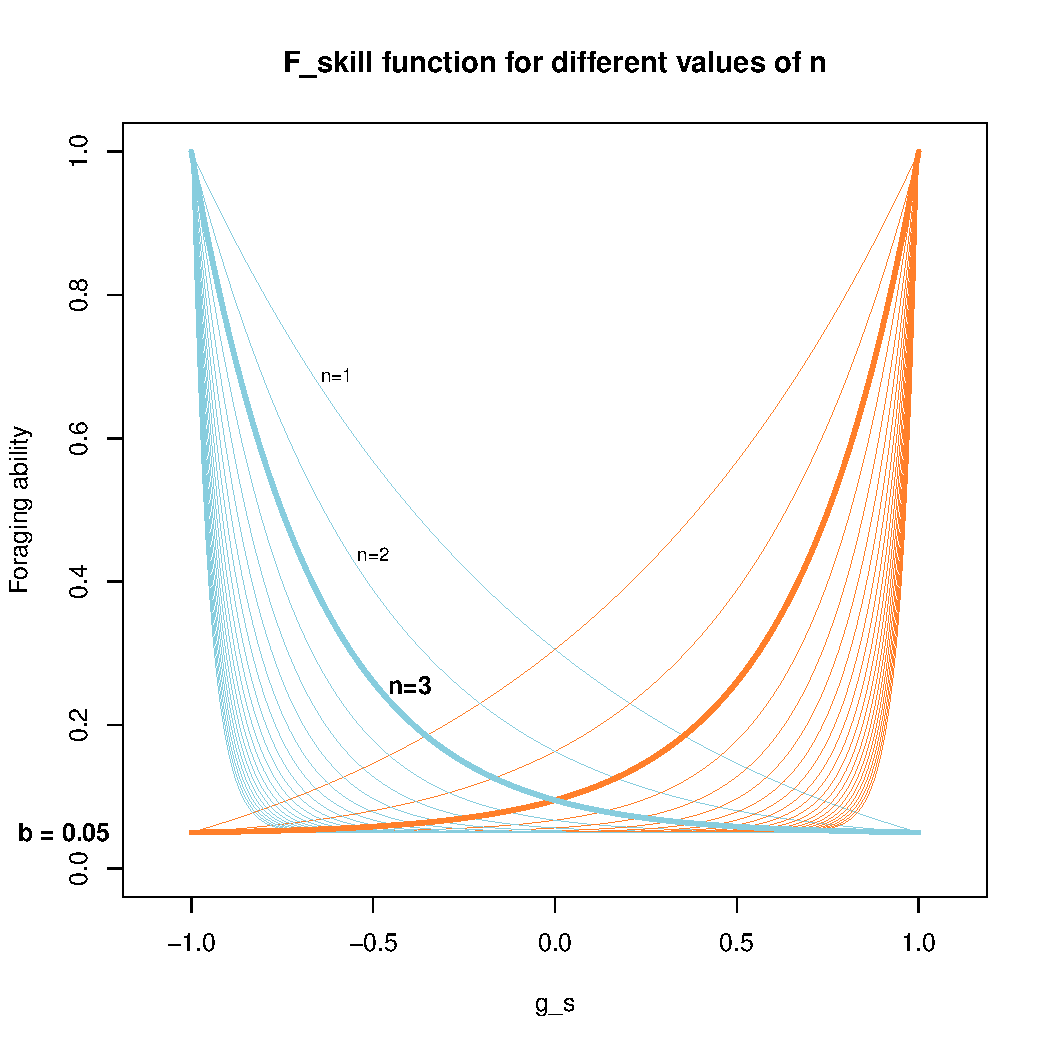
\includegraphics[height=5.5cm]{images/f_skill_alpha}
	\end{figure}
	
	
	\column{0.50\textwidth}
	$$ f_{skill}(g_{s,i},type_Q)= {\frac{\left(e^{n*g_{s,i}*t_q}\right)+C(b,n)} {e^{n}+C(b,n)}}$$
	\begin{enumerate}
	\item[ $\rightarrow$] Tune $f_{skill}$ : $n=?$, $b=?$
	% 	\item Fix $\alpha$ to force specialization.
	\end{enumerate}
	
	\end{columns}
	
	
	\end{frame}
	%%%----------------------------------------------------------------------
	%%%----------------------------------------------------------------------
	
	\begin{frame}{Add a density pressure}\addtocounter{framenumber}{-1}
	
	$$F_{rwd,t}(i,Q) = f_{skill}\left(g_{s,i},T_Q\right)\times d_{penality}\left(h_{Q,t}\right)\times \alpha$$
	
	\begin{columns}
	
	\column{0.50\textwidth}
	
	
	\begin{itemize}
	\item $i$ the agent,
	\item $t$ the iteration of the simulation,
	\item $ d_{penality}(h_{Q,t}) =  1 - \frac {h_{Q,t}} {nrobots} $
	\item $ f_{skill}(g_{s,i},type_Q)= {\left(e^{n*g_{s,i}*t_q}\right)+C(b,n) \over {e^{n}+C(b,n)}}$
	\item $h_{Q,t} \in [0, n -1]$ the number of robot harvesting $Q$ at $t$ 
	\item $g_{s,i} \in [-1,1]$ the value of the gene for the foraging skill of $i$,
	\item $T_Q\in \{-1,1\}$ the type of the resource Q
	\item $ C(b,n) = {(be^{n} - e^{-n} )\over{(1-b)}} $
	\end{itemize}
	
	
	% where  , $n$ and $C(b)$ are two parameters allowing us to tunes the environment hostility.
	
	
	
	
	
	\column{0.50\textwidth}
	
	\begin{figure}
	\includegraphics[height=5.5cm]{images/densite}
	\end{figure}
	
	
	\end{columns}
	
	
	\end{frame}
	
	
	\end{document}
	